\documentclass[11pt]{article}

\usepackage[margin=1in]{geometry}
\usepackage{amsmath,amssymb,amsthm}
\usepackage{tikz}
\usetikzlibrary{arrows.meta}
\usepackage{booktabs}
\usepackage{microtype}
\usepackage[hidelinks]{hyperref}
\usepackage{url}

\newcommand{\R}{\mathbb{R}}
\newcommand{\Q}{\mathbb{Q}}
\DeclareMathOperator*{\argmin}{arg\,min}

\theoremstyle{plain}
\newtheorem{theorem}{Theorem}
\newtheorem{lemma}{Lemma}
\newtheorem{corollary}{Corollary}
\theoremstyle{remark}
\newtheorem*{remark}{Remark}

\title{Exact-Rational Certificates in Podium:\\
Constructions, Proofs, and Prior Art\\
{\large A technical note}}
\author{Adi Oltean\thanks{Starcloud, Inc. Companion to the repository
\texttt{github.com/adi-oltean/podium}. This is a technical note documenting the
exact-arithmetic certificates in \texttt{podium.verify} and their proofs; it is
not a submission and claims no new mathematics (see the positioning at the end of
Section~\ref{sec:discipline}).}}
\date{July 2026}

\begin{document}
\maketitle

\begin{abstract}
This note collects the constructions, proofs, and prior-art positioning behind
the exact-rational certificates in the Podium library (\texttt{podium.verify}):
barrier certificates for abort safety, Karush--Kuhn--Tucker certificates for the
online convex solves, control-Lyapunov certificates, sum-of-squares certificates,
and an optimality-gap bracket for nonconvex quadratically constrained quadratic
programs. None of the underlying mathematics is new; the note documents the exact
instantiation, its verification, and its relation to the
exact-SOS/moment, rational-SDP-recovery, and QCQP-duality literature, so that a
math-inclined reader can audit the certificate layer directly. Each result is
exercised by a test in the repository. In detail, guidance and control software
relies on numerical optimization and floating-point synthesis whose executions
are difficult to verify directly. We study the problem of verifying solver
\emph{outputs}: given a certificate produced by an untrusted floating-point
solver, we re-verify it in exact rational arithmetic, so that acceptance
constitutes a proof that carries no rounding error. We apply this method to four
properties: abort safety, via
barrier certificates; optimality of the online convex solves, via
Karush--Kuhn--Tucker (KKT) conditions for quadratic and second-order cone
programs; closed-loop stability, via Lyapunov ellipsoids from a discrete-time
linear-quadratic regulator; and polynomial set containment, via sum-of-squares
certificates. These certificates are standard; we give exact re-verification
procedures --- tolerance-free for the barrier, Lyapunov, sum-of-squares, and
optimality-gap certificates, and an exact suboptimality bound for the KKT
re-check of an approximate online solve --- and a reference implementation.

For nonconvex quadratically constrained quadratic programs (QCQPs), we specialize
the exact rational recovery of a semidefinite certificate, developed for
polynomial optimization by Peyrl and Parrilo and by Kaltofen et al., to the
S-procedure dual. This yields a tolerance-free, machine-checkable optimality-gap
bracket: a rational lower bound from the S-procedure dual and a rational upper
bound from a feasible point, coinciding exactly at a global optimum. Our analytic
contribution is a characterization of how the certified lower bound degrades
under rational rounding of the dual multiplier: the value loss is second-order in
the rounding denominator in the nonsingular case and first-order in the
trust-region hard case, with soundness retained in both, and it vanishes when the
optimal multiplier is rational (Theorems~\ref{thm:recovery} and~\ref{thm:hard}).
For several constraints the S-procedure need not be tight, and the bracket then
certifies a duality gap with both endpoints exact (Theorem~\ref{thm:multi}). Each
result is accompanied by a verifying test in the reference implementation.
\end{abstract}

\section{Introduction}

Software increasingly makes consequential decisions by solving optimization
problems numerically. A spacecraft plans a fuel-optimal approach; a controller
selects a maneuver that must avoid a keep-out zone; an autopilot commits to a
command computed by a convex solver. In each case the solver returns an answer,
but the answer is a floating-point number produced by an opaque computation
rather than a proof that the answer is correct or optimal. Floating-point
arithmetic rounds at every step, and a computation that appears to succeed can
return a value that is subtly wrong. Where a mistake is costly and cannot be
undone after the fact, as in spaceflight, it is desirable for the solver's
answer to carry a \emph{certificate}: a small, separate object that an
independent program can verify exactly, so that correctness rests on the
verifier rather than on the solver. This paper constructs such certificates for
guidance and control, and studies in particular the problem of certifying that a
computed trajectory is close to the best one achievable.

A concrete instance motivates the main results. Nonconvex trajectory
optimization for rendezvous, atmospheric entry, and powered landing is commonly
solved by successive convexification, which linearizes the nonconvex constraints
about the current iterate and solves a convex subproblem, repeating until
convergence \cite{elango2025}. The method returns a feasible
trajectory, but that trajectory is only locally optimal, and the solver reports
its cost as a floating-point number rather than a bound on the global optimum.
The method thus provides no bound on the distance between the computed cost and
the global optimum. This paper supplies such a bound: an exact-arithmetic
certificate that brackets the global optimum, so that the suboptimality of a
computed solution is certified rather than assumed, and, when the bracket
closes, the solution is certified globally optimal. The certificate requires
neither convexity nor trust in the solver.

The underlying idea is general. A guidance and control stack executes a large
amount of untrusted
numerical code: convex solvers compute commands, semidefinite programs (SDPs)
synthesize safety and stability certificates, and floating-point routines emit
actuator signals. Verifying the \emph{execution} of these components, including
worst-case iteration counts and bitwise solver behavior, is difficult and often
impractical \cite{arnstrom2022}. We instead verify the \emph{answer}: an
untrusted floating-point tool proposes a certificate, and a trusted checker
re-establishes the property in exact rational arithmetic, without floating-point
computation of its own. Because the check is a short, deterministic computation,
it can be re-run automatically whenever the code or data change. This matters in
practice: a candidate certificate produced in floating point may satisfy its
defining condition only approximately, so a tolerance-based check can accept a
pair $(\lambda, t)$ whose value $t$ exceeds the true optimum, whereas the exact
rational test accepts a certificate only when it holds exactly.

\paragraph{Contributions.}
\begin{enumerate}\itemsep2pt
\item An exact-rational verification layer for four standard guidance and
control certificates, barrier abort safety, Karush--Kuhn--Tucker (KKT)
optimality of the online convex solves, Lyapunov stability, and sum-of-squares
set containment (Section~\ref{sec:family}), each synthesized by an untrusted
solver and re-checked over the rationals $\Q$ (exactly, or within an explicit
rational bound for the approximate online solves).
\item A specialization of exact rational SDP-certificate recovery to the
S-procedure dual of a nonconvex quadratically constrained quadratic program
(QCQP), giving a tolerance-free machine-checkable optimality-gap bracket for
guidance and control (Section~\ref{sec:bracket}). This furnishes the certified
global-suboptimality bound that a successive convexification solution does not
carry (Section~\ref{sec:scvx}).
\item A rounding-rate analysis of that bracket: the certified lower bound loses
value at second order in the rounding denominator in the nonsingular case
(Theorem~\ref{thm:recovery}) and at first order in the trust-region hard case
(Theorem~\ref{thm:hard}), with soundness retained in both, and the bracket
certifies an exact duality gap when the S-procedure is not tight
(Theorem~\ref{thm:multi}).
\item An open reference implementation whose trusted checker uses no floating
point, in which each result is exercised by a test that reconstructs the
certificate over $\Q$ (Section~\ref{sec:impl}).
\end{enumerate}

None of the underlying certificates is new. The barrier certificates are due to
Prajna and Jadbabaie \cite{prajna2004} and Ames et al.\ \cite{ames2017}; the
Lyapunov re-verification follows Wang et al.\ \cite{feron2013}; the S-lemma is
due to Yakubovich \cite{yakubovich1971} and its exactness is surveyed by P\'olik
and Terlaky \cite{polik2007}. Most importantly, the recovery of an exact rational
certificate from a floating-point SDP solution, and its use to certify global
lower bounds in polynomial optimization, is due to Peyrl and Parrilo
\cite{peyrl2008}, Kaltofen et al.\ \cite{kaltofen2012}, and Magron and Safey El
Din \cite{magron2018}; Davis and Papp \cite{davis2022} recover exact rational
certificates directly from a numerical dual certificate and prove a convergence
rate, and rigorous bracketing of a relaxation value is provided by verified SDP
\cite{jansson2009,roux2018}. A nonconvex QCQP is the degree-two case of this
machinery, and its exactness and hidden convexity are themselves classical
\cite{bental1996,beck2006,polik2007}. Our contribution is therefore not exact
rational certification, the bracket idea, nor certificate recovery with a rate,
but the specialization of these to the S-procedure dual of a QCQP, in particular
the second-order (nonsingular) versus first-order (trust-region hard case)
rounding-rate dichotomy of Section~\ref{sec:bracket}, together with a
tolerance-free implementation for a guidance and control verification stack.

\section{Exact re-verification of solver output}
\label{sec:discipline}

A \emph{certificate} is a small object that makes a property easy to confirm even
when the property was hard to establish: a Lyapunov matrix for stability, a
multiplier for a bound, a sum-of-squares decomposition for nonnegativity. Our
method separates search from proof. An untrusted floating-point routine searches
for the certificate, typically by solving an SDP or an interior-point problem.
The result is then rounded to nearby rational numbers and checked by an exact
computation over $\Q$.

The single trusted primitive is an exact test for positive semidefiniteness
(PSD), a symmetric $LDL^\top$ elimination over $\Q$ in $O(n^3)$ operations: a
symmetric matrix is PSD if and only if every pivot is nonnegative and each zero
pivot leaves the rest of its row, and hence by symmetry its column, in the Schur
complement zero. The resulting factorization $M = L D L^\top$ with $D \succeq 0$
is itself the nonnegativity witness, since $z^\top M z = \sum_i D_{ii}
(l_i^\top z)^2$. This avoids eigenvalues, which are in general irrational and
admit no exact rational representation, and the leading-minor test of Sylvester,
which certifies strict definiteness only. The trusted checker uses only exact
rational arithmetic, so its conclusions carry no rounding error. For the barrier, Lyapunov, sum-of-squares, and optimality-gap
certificates, acceptance is an exact identity together with the PSD test, with no
tolerance. When the object under test is the output of an approximate solver, as
for the online convex solves below, the residuals are still computed exactly, but
a rigorous bound on suboptimality is reported only when those exact residuals
yield a valid Lagrangian dual point, not merely when they are small.

\section{Four certificate families}
\label{sec:family}

\paragraph{Barrier certificates for abort safety.}
For linearized relative motion with a spherical keep-out zone, an SDP produces a
barrier function whose sublevel set is invariant under the passive, thrust-free
drift. The checker verifies over $\Q$ an S-procedure condition, in which a
nonnegative multiplier certifies that one quadratic is nonnegative on the zero
set of another, together with an exactly vanishing Lie derivative, the rate of
change of the barrier along the drift. Together these establish forward
invariance of the safe set, so that the abort set never intersects the keep-out
zone \cite{prajna2004,ames2017}.

\paragraph{KKT certificates for the online solves.}
The guidance layer solves a quadratic program (QP) and a second-order cone
program (SOCP) online. The solver returns an approximate primal-dual point, and
the checker computes its KKT residuals, stationarity, primal and dual
feasibility, and complementary slackness, exactly. A small stationarity residual
is not by itself a bound on suboptimality: with a rank-deficient objective (a
linear or minimum-fuel program) an approximately stationary point can be
arbitrarily far from optimal. The checker therefore reports a rigorous bound only
when a valid Lagrangian dual point exists, namely when the multiplier is
dual-feasible, the Hessian $P$ is PSD, and the stationarity residual $r$ lies in
the range of $P$. The exact gap
$\mu^\top(h - Gx) + \nu^\top(b - Ax) + \tfrac12\, r^\top P^{+} r$ then bounds
$p(x) - p^\star$, the term $\tfrac12\, r^\top P^{+} r$ being the objective drop
from the candidate to the exact minimizer of the Lagrangian, computed by solving
$P z = r$ over the rationals. A SOCP objective is linear and so has no curvature
to absorb a residual; a rigorous bound there instead requires exact conic-dual
feasibility. Membership of a slack vector
$s = (s_0, s_{1:}) \in \R \times \R^d$ in the second-order cone is decided without
square roots through the algebraic condition $s_0 \ge 0$ and
$\lVert s_{1:}\rVert^2 \le s_0^2$. In every case the checker verifies that the
objective Hessian is PSD, so that the certificate concerns a global optimum of a
convex program rather than a stationary point of unknown type.

\paragraph{Lyapunov certificates for closed-loop stability.}
A cost-to-go matrix $P$ from a discrete-time linear-quadratic regulator (LQR) is
re-verified as positive definite, so that its sublevel sets are bounded
ellipsoids, and as satisfying the Lyapunov decrease condition
$P - A_{\mathrm{cl}}^\top P A_{\mathrm{cl}} \succeq 0$, where
$A_{\mathrm{cl}} = A - BK$ is the closed-loop transition matrix under the
state-feedback gain $K$, using the same exact PSD test, in the sense of
\cite{feron2013}.

\paragraph{Sum-of-squares (SOS) certificates for set containment.}
The nonnegativity of a polynomial $p(x)$, for instance that a certified attitude
cone contains a given sublevel set, is verified as an identity
$p(x) = z(x)^\top G\, z(x)$ with $G$ symmetric positive semidefinite, where
$z(x)$ is a vector of monomials and $G$ is the associated Gram matrix. Such a
representation exhibits $p$ as a sum of squares, and hence as nonnegative. The Gram matrix is recovered from an approximate SDP
solution by the rational rounding of Peyrl and Parrilo \cite{peyrl2008} and Roux
et al.\ \cite{roux2018}.

\section{Optimality-gap bounds for nonconvex QCQPs}
\label{sec:bracket}

Quadratically constrained quadratic programs arise throughout guidance: keep-out
zones, thrust limits, and
terminal sets are quadratic, and each convex subproblem inside a
successive convexification loop is a convex QCQP or its second-order cone
relaxation.
When the constraints are nonconvex the problem is NP-hard in general, and a
solver can return a feasible point but not, on its own, a proof that no better
point exists. We construct such a proof in exact arithmetic: a lower bound $t$
and an upper bound $u$ with $t \le J^\star \le u$, both rational and both checked
without floating point, so that $u - t$ is a certified optimality gap and the
case $t = u$ certifies a global optimum (Figure~\ref{fig:bracket}).

Consider the QCQP
\begin{equation}
J^\star = \inf_{x \in \R^n}\Big\{ f_0(x) : f_k(x) \ge 0,\ k = 1, \dots, m \Big\},
\qquad f_j(x) = x^\top P_j x + q_j^\top x + r_j,
\label{eq:qcqp}
\end{equation}
with symmetric $P_j$. A keep-out constraint $\lVert x - c \rVert \ge R$ renders
the feasible set nonconvex. Throughout we use the instance
$\min \lVert x \rVert^2$ subject to $\lVert x - (3,0) \rVert \ge 5$, whose origin
lies inside the excluded ball; its global optimum is $J^\star = 4$, attained at
$(-2, 0)$ with multiplier $\lambda^\star = 2/5$. Table~\ref{tab:results} lists
this and the other cases considered below.

\subsection{The bracket and its soundness}

The lower bound is a Lagrangian relaxation, certified exactly. For multipliers
$\lambda \in \R^m_{\ge 0}$ the Lagrangian
$L(x, \lambda) = f_0(x) - \sum_k \lambda_k f_k(x)$ is quadratic in $x$, and with
the homogenized coordinate $z = [x; 1] \in \R^{n+1}$ the shifted form
$L(x, \lambda) - t$ equals $z^\top M(\lambda, t) z$, where
\begin{equation}
M(\lambda, t) = \begin{bmatrix}
P_0 - \sum_k \lambda_k P_k & \tfrac12(q_0 - \sum_k \lambda_k q_k) \\[2pt]
\tfrac12(q_0 - \sum_k \lambda_k q_k)^\top & r_0 - \sum_k \lambda_k r_k - t
\end{bmatrix}.
\label{eq:M}
\end{equation}

\begin{theorem}[Lower bound]\label{thm:sound}
If $\lambda \ge 0$ componentwise and $M(\lambda, t) \succeq 0$, then
$t \le J^\star$.
\end{theorem}
\begin{proof}
For any $x$, writing $z = [x; 1]$, expansion gives
$z^\top M(\lambda, t) z = f_0(x) - \sum_k \lambda_k f_k(x) - t$. Positive
semidefiniteness of $M$ makes this nonnegative for all $x$. At a feasible $x$,
each $f_k(x) \ge 0$ and each $\lambda_k \ge 0$, so
$\sum_k \lambda_k f_k(x) \ge 0$ and hence $f_0(x) \ge t$. Taking the infimum over
feasible $x$ gives $t \le J^\star$.
\end{proof}

The argument is Lagrangian weak duality and uses no convexity, constraint
qualification, or boundedness. Conversely, on the primal side, any point
$\bar x$ with $f_k(\bar x) \ge 0$ for all $k$ gives $J^\star \le f_0(\bar x)$. The
feasibility of $\bar x$ must be checked exactly: a point that is feasible only
within a solver tolerance may have objective value below $J^\star$, which would
place the upper bound below the true optimum. The checker therefore evaluates
$f_k(\bar x) \ge 0$ over the rationals. By elementary gap closure, if a certified
lower bound $t$ equals a certified upper bound $u = f_0(\bar x)$ then
$J^\star = t = u$, an exact certificate of the global optimum. The two bounds are
the rationalized Shor/S-procedure lower bound and a rational feasible point,
standard ingredients of verified global optimization; the content of this section
is their specialization to the QCQP dual and the rounding-rate analysis below.

\begin{figure}[t]
\centering
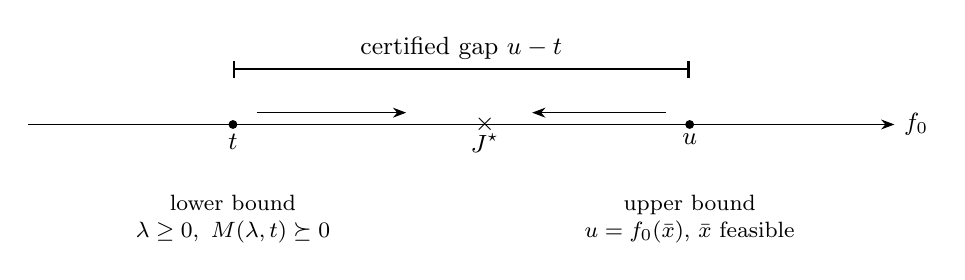
\begin{tikzpicture}[font=\small, >={Stealth[]}]
\draw[->] (-0.4,0) -- (10.6,0) node[right] {$f_0$};
\coordinate (t) at (2.2,0);
\coordinate (js) at (5.4,0);
\coordinate (u) at (8.0,0);
\fill (t) circle (1.6pt);
\fill (u) circle (1.6pt);
\draw (js) node {$\times$};
\draw[|-|, thick] (2.2,0.7) -- (8.0,0.7)
  node[midway, above] {certified gap $u-t$};
\node[below] at (t) {$t$};
\node[below] at (js) {$J^\star$};
\node[below] at (u) {$u$};
\node[align=center, font=\footnotesize] at (2.2,-1.2)
  {lower bound\\ $\lambda\ge0,\ M(\lambda,t)\succeq0$};
\node[align=center, font=\footnotesize] at (8.0,-1.2)
  {upper bound\\ $u=f_0(\bar x)$, $\bar x$ feasible};
\draw[->] (2.5,0.15) -- (4.4,0.15);
\draw[->] (7.7,0.15) -- (6.0,0.15);
\node[font=\footnotesize] at (5.1,0.2) {\phantom{x}};
\end{tikzpicture}
\caption{The bracket. A rational multiplier with $M(\lambda,t)\succeq0$ gives a
certified lower bound $t\le J^\star$; an exactly feasible point gives a certified
upper bound $u=f_0(\bar x)\ge J^\star$. Both are exact rationals, so $u-t$ is a
certified optimality gap; when $t=u$ the global optimum is certified exactly. The
arrows indicate refinement of the dual and of the feasible point.}
\label{fig:bracket}
\end{figure}

\subsection{Recovery of an exact bound from an approximate dual}

Fix $m = 1$ and write $A(\lambda) = P_0 - \lambda P_1$, $b = q_0 - \lambda q_1$,
$c = r_0 - \lambda r_1$, and $g(\lambda) = \inf_x (f_0 - \lambda f_1)$ on the set
$U = \{\lambda : A(\lambda) \succ 0\}$.

\begin{lemma}\label{lem:schur}
For $\lambda \in U$, $g(\lambda) = c - \tfrac14 b^\top A(\lambda)^{-1} b$, and
$M(\lambda, t) \succeq 0$ if and only if $t \le g(\lambda)$.
\end{lemma}
\begin{proof}
On $U$ the quadratic $f_0 - \lambda f_1 = x^\top A x + b^\top x + c$ is strictly
convex, with unique minimizer $x^\star = -\tfrac12 A^{-1} b$ and minimum value
$g(\lambda) = c - \tfrac14 b^\top A^{-1} b$. Since $A \succ 0$, the Schur
complement\footnote{For a block matrix $\left[\begin{smallmatrix} A & v \\
v^\top & d \end{smallmatrix}\right]$ with $A \succ 0$, positive semidefiniteness
is equivalent to nonnegativity of the scalar Schur complement
$d - v^\top A^{-1} v$.} of $A$ in $M(\lambda, t)$ is
$(c - t) - \tfrac14 b^\top A^{-1} b$, and $M(\lambda, t) \succeq 0$ if and only
if this is nonnegative, that is, $t \le g(\lambda)$.
\end{proof}

By Cramer's rule $g$ is a rational function of $\lambda$ with coefficients
rational in the problem data, so a rational $\lambda \in U$ yields a rational,
and therefore exactly certified, lower bound. For a single constraint with a
strictly feasible point, the S-lemma gives strong duality,
$J^\star = \max_{\lambda \ge 0} g(\lambda) = g(\lambda^\star)$
\cite{yakubovich1971}.

\begin{theorem}[Nonsingular recovery]\label{thm:recovery}
Suppose $A(\lambda^\star) \succ 0$. Then $g$ is smooth and concave near
$\lambda^\star$ with $g'(\lambda^\star) = 0$, so
$J^\star - g(\lambda) = O((\lambda - \lambda^\star)^2)$. Rounding $\lambda^\star$
to a rational $\lambda$ with denominator at most $D$, so that
$|\lambda - \lambda^\star| \le 1/D$, yields an exactly certified lower bound with
$J^\star - g(\lambda) = O(1/D^2)$. If in addition $\lambda^\star$ and $J^\star$
are rational, then $(\lambda^\star, J^\star)$ is an exact certificate, and with a
rational optimizer the bracket closes exactly.
\end{theorem}
\begin{proof}
On $U$, $g$ is a rational function, hence smooth, and is concave as an infimum of
functions affine in $\lambda$. At an interior maximizer $g'(\lambda^\star) = 0$,
so Taylor's theorem gives
$J^\star - g(\lambda) = \tfrac12 |g''(\xi)| (\lambda - \lambda^\star)^2$ for some
$\xi$ between $\lambda$ and $\lambda^\star$. Substituting
$|\lambda - \lambda^\star| \le 1/D$ gives the $O(1/D^2)$ bound. Exactness of
$g(\lambda^\star)$ when $\lambda^\star$ is rational follows from
Lemma~\ref{lem:schur}.
\end{proof}

\begin{remark}
With several constraints, an interior maximizer means interior with respect to
the active constraints. The stationarity $\partial g / \partial \lambda_k = 0$
holds for active multipliers ($\lambda_k^\star > 0$); an inactive constraint sits
at $\lambda_k^\star = 0$ on the boundary of the nonnegative orthant, where the
corresponding derivative is negative.
\end{remark}

In the reference implementation, rounding an approximate dual value
$\tilde\lambda \approx 0.4003$ for the running instance to a denominator at most
$100$ recovers $\lambda^\star = 2/5$ and $t = 4 = J^\star$ exactly.

\subsection{The singular case}

\begin{theorem}[Singular recovery]\label{thm:hard}
Suppose $A(\lambda^\star)$ is positive semidefinite but singular, the
trust-region hard case \cite{moresorensen1983}. Then:
(a) if $\lambda^\star$ and $J^\star$ are rational, $(\lambda^\star, J^\star)$ is
an exact certificate, since $M$ is a rank-deficient PSD matrix that the exact
test accepts, so soundness is unaffected;
(b) approaching $\lambda^\star$ from within $U$ gives certified rational lower
bounds that converge to $J^\star$ linearly;
(c) exact closure requires $\lambda^\star$ and $J^\star$ to be rational, which
does not hold generically, as $J^\star$ may be algebraic of degree greater
than one.
\end{theorem}
\begin{proof}
(a) Soundness is Theorem~\ref{thm:sound}, which requires only $\lambda^\star \ge
0$ and $M(\lambda^\star, J^\star) \succeq 0$; the exact $LDL^\top$ test accepts a
rank-deficient PSD matrix, since at a zero pivot the rest of the row vanishes and
the elimination continues with a nonnegative $D$.
(b) Since $A \succ 0$ on $U$ and $A(\lambda^\star)$ is singular, $\lambda^\star$
lies on the boundary of $U$. On $U$, $g$ is the smooth concave function of
Lemma~\ref{lem:schur}, and $J^\star = \sup_{\lambda \ge 0} g$ is attained at
$\lambda^\star$ on that boundary. A boundary maximizer need not be stationary, so
the right derivative
$g'_+(\lambda^\star) := \lim_{\lambda \downarrow \lambda^\star} g'(\lambda)$ is
generically nonzero, and a first-order expansion gives
$J^\star - g(\lambda) = |g'_+(\lambda^\star)| \, |\lambda - \lambda^\star| +
o(|\lambda - \lambda^\star|)$, which is linear. This contrasts with
Theorem~\ref{thm:recovery}, where an interior maximizer forces
$g'(\lambda^\star) = 0$ and a quadratic rate.
(c) Here $\lambda^\star$ solves $\det A(\lambda) = 0$ together with the boundary
optimality condition, so it may be algebraic of degree greater than one, and
rationality of $\lambda^\star$ and $J^\star$ fails in general.
\end{proof}

Soundness is thus retained in the singular case; only the recovery rate falls.
The implementation's instance $\min -x_1^2 + 2 x_2^2 + 2 x_2$ subject to
$1 - \lVert x \rVert^2 \ge 0$ has
$A(\lambda) = \operatorname{diag}(-1 + \lambda,\, 2 + \lambda)$, singular at
$\lambda^\star = 1$, with $J^\star = -4/3$. The certified gap decreases by one
order of magnitude for each order of magnitude of $|\lambda - 1|$, consistent
with the linear rate, compared with two orders in the nonsingular case. An exact rational
recovery in the singular case, by a pseudoinverse together with a Diophantine
argument in the manner of the rank-deficient case of \cite{peyrl2008}, remains
open.

\subsection{Several constraints}

\begin{theorem}[Certified duality gap]\label{thm:multi}
Theorem~\ref{thm:sound} and the closing observation hold for every $m$. Let
$d^\star$ be the Shor relaxation value of \eqref{eq:qcqp}, that is, the supremum
of $t$ over rational $\lambda \ge 0$ and $t$ with $M(\lambda, t) \succeq 0$. Then
$d^\star \le J^\star$ always, and for $m \ge 2$ this inequality may be strict.
When it is, any certified lower bound $t \le d^\star$ and any exactly feasible
$\bar x$ give an interval $[t, f_0(\bar x)]$ that contains $J^\star$, with both
endpoints exact rationals and $f_0(\bar x) - t > 0$ a certified duality gap.
\end{theorem}

\begin{remark}
For $m = 1$ with a strictly feasible point the S-lemma gives $d^\star = J^\star$,
so the bracket can close (Theorem~\ref{thm:recovery}). For $m \ge 2$ this strong
duality may fail. Higher levels of the moment hierarchy of Lasserre
\cite{lasserre2001} then give nondecreasing certified lower bounds converging to
$J^\star$ under a compactness (Archimedean) condition, each verified by an exact
PSD test.
\end{remark}

The soundness argument is that of Theorem~\ref{thm:sound} with the sum taken over
$m$ constraints. In a sweep of
forty random two-constraint instances of Celis--Dennis--Tapia type,\footnote{The
Celis--Dennis--Tapia problem minimizes a quadratic over the intersection of two
quadratic constraints; it is the standard example in which the Shor relaxation
can be inexact.} seven exhibited a strictly positive Shor gap, the largest equal
to $1.72$. In each such case the bracket encloses a nonconvex optimum with no
closed form, with both endpoints verified over $\Q$.

\subsection{Relation to successive convexification}
\label{sec:scvx}

Nonconvex trajectory optimization in guidance is commonly addressed by successive
convexification and sequential convex programming, which solve a nonconvex
program by repeatedly convexifying about the current iterate and solving a convex
subproblem \cite{elango2025,acikmese2011}. Such methods return a feasible
trajectory that is locally optimal, without a bound on its distance from the
global optimum. The bracket supplies that bound. A converged iterate $\bar x$ is
a feasible point, hence a certified upper bound $u = f_0(\bar x)$
(Theorem~\ref{thm:sound}); the S-procedure dual of Section~\ref{sec:bracket}
supplies a certified lower bound $t$ for the same problem; and $[t, u]$ is a
bound on the global suboptimality of the trajectory, with $u - t$ its certified
gap, all verified over $\Q$. When the bracket closes, the trajectory is certified
globally optimal; when it does not, the residual gap $u - t$ is still a certified
bound on suboptimality, and Theorem~\ref{thm:multi} identifies cases in which the
lower bound cannot be tight. We establish this on the keep-out QCQP, the
nonconvex primitive that these methods convexify;
extending the exact certificate from that primitive to full trajectory horizons
is the principal open problem (Section~\ref{sec:limits}).

\section{Reference implementation}
\label{sec:impl}

\begin{table}[t]
\centering
\caption{Representative instances. All certified bounds are exact rationals
verified over $\Q$; ``closed'' indicates that the certified lower bound $t$ and
upper bound $u$ coincide and hence certify $J^\star$. The value
$\tilde\lambda \approx 0.4003$ is the approximate dual fed to the rational
rounding step; the recovered certificate is exact.}
\label{tab:results}
\begin{tabular}{@{}llccc@{}}
\toprule
Instance & Case & $\lambda^\star$ & certified $[t,\,u]$ & $J^\star$ \\
\midrule
$\min\lVert x\rVert^2$, $\lVert x-(3,0)\rVert\ge5$ & nonsingular, closed & $2/5$ & $[4,\,4]$ & $4$ \\
\quad same, non-optimal upper point & open bracket & $2/5$ & $[4,\,169/25]$ & $4$ \\
recovery from $\tilde\lambda\approx0.4003$ & quadratic rate & $2/5$ & $t=4$ & $4$ \\
$\min -x_1^2{+}2x_2^2{+}2x_2$, $\lVert x\rVert\le1$ & singular & $1$ & $[-4/3,\,-4/3]$ & $-4/3$ \\
two active keep-outs & several constraints & $(\tfrac12,\tfrac12)$ & $[5,\,5]$ & $5$ \\
Celis--Dennis--Tapia sweep (7 of 40) & duality gap & \text{--} & $u-t\le1.72$ & \text{--} \\
\bottomrule
\end{tabular}
\end{table}

The certificates and theorems above are implemented in a reference library whose
trusted checker uses only exact rational arithmetic. Each theorem is exercised by
a test that
constructs the certificate and re-verifies it over $\Q$; the representative
cases are collected in Table~\ref{tab:results}. Two requirements that a
tolerance-based check would miss are enforced exactly. First, the checker
verifies feasibility of $\bar x$ over the rationals, since a point feasible only
within a tolerance may have objective value below $J^\star$. Second, the closing
criterion draws its two bounds from a single problem instance, since bounds
computed for different instances cannot be compared.

\section{Related work}

Exact and certified certificates for global polynomial optimization are an
established subject. The moment/SOS hierarchy of Lasserre \cite{lasserre2001} and
Parrilo \cite{parrilo2003} gives convergent certified lower bounds, Henrion and
Lasserre \cite{henrion2005} extract optimizers and detect global optimality, and
Nie, Demmel, and Sturmfels \cite{nie2006} give SOS exactness over the gradient
ideal. Exact rational certificates recovered from a numerical SDP are due to
Peyrl and Parrilo \cite{peyrl2008}, Kaltofen et al.\ \cite{kaltofen2012}, and
Magron and Safey El Din \cite{magron2018}; closest to our rate statement, Davis
and Papp \cite{davis2022} construct exact rational certificates from numerical
dual certificates and prove a convergence rate. Rigorous, though not exact,
bracketing of the relaxation value by verified SDP is due to Jansson
\cite{jansson2009} and Roux et al.\ \cite{roux2018}, and an exact SDP duality
theory to Ramana \cite{ramana1997}. A nonconvex QCQP is the degree-two instance
of this machinery; its duality, exactness, and hidden convexity are classical
\cite{yakubovich1971,shor1987,polik2007,bental1996,beck2006,jeyakumar2014}, as is
the trust-region hard case \cite{moresorensen1983,adachi2017}.

Against this background our contribution is narrow. We instantiate the exact
rational recovery of Peyrl and Parrilo and of Davis and Papp on the S-procedure
dual matrix $M(\lambda,t)$ of a QCQP; we record the rounding rate of the
resulting certified lower bound, second-order in the nonsingular case
(Theorem~\ref{thm:recovery}) and first-order in the trust-region hard case
(Theorem~\ref{thm:hard}). This is the standard second-order-versus-first-order
behavior of rounding at an interior as against a boundary maximizer, stated for
the QCQP dual; we do not claim it as new. The weak-duality bracket and its
closure are likewise standard. The contribution is the integration: a
tolerance-free, exact-rational instantiation of this machinery, wired into a
guidance and control verification stack (Section~\ref{sec:scvx}) and re-checked
automatically. Barrier and control-barrier
certificates \cite{prajna2004,ames2017}, credible autocoding \cite{feron2013},
and the verification of convex-optimization solvers for model-predictive control
\cite{cohen2020} are complementary in verifying control software: the last
verifies the solver algorithm, whereas we verify its output. Lossless
convexification \cite{acikmese2011} and successive convexification
\cite{elango2025} address the feasibility and tightness of convex reformulations;
the optimality-gap bounds here certify the global suboptimality of the resulting
trajectory (Section~\ref{sec:scvx}).

\section{Limitations and open problems}
\label{sec:limits}

The lower-bound soundness of Theorems~\ref{thm:sound} and~\ref{thm:multi} and the
nonsingular recovery of Theorem~\ref{thm:recovery} are complete. An exact
rational recovery in the singular case (Theorem~\ref{thm:hard}) and an exact
higher-level moment certificate for the multi-constraint gap
(Theorem~\ref{thm:multi}) remain open. The $LDL^\top$ PSD test is $O(n^3)$, so
the barrier to trajectory-scale certificates is not the test but the growth of
the rational entries under exact elimination. The matrices of a discretized
trajectory problem are block-banded, and a fraction-free elimination that
exploits that structure would bound the certificate bit-size in the horizon; a
structure-exploiting exact certificate at trajectory scale is the natural next
step.

\section{Conclusion}

We have described a method that verifies the output of untrusted guidance and
control computation
in exact rational arithmetic, and applied it to barrier safety, KKT optimality,
Lyapunov stability, and sum-of-squares set containment. Its technical content
specializes exact rational SDP-certificate recovery to the S-procedure dual of a
nonconvex QCQP, and characterizes the rounding rate of the certified lower bound,
which is second-order in the nonsingular case and first-order in the trust-region
hard case, with soundness retained in both, and a certified exact duality gap
when the relaxation is not tight. The constructions are realized in an open
reference implementation.

\bibliographystyle{unsrt}
\bibliography{references}

\end{document}
